\chapter{Model set-up}

\section{Introduction}

\section{The CSF PCRaster format}

Ech2o reads spatial information using the binary raster format (cross-system format, CSF) used in the free GIS PCRaster\footnote{Downloadable for free at http://pcraster.geo.uu.nl/} . By using this format, full GIS capability for data pre-processing, post-processing and visualization is added to \echo.

\section{The configuration file}

The configuration file is the main communication interface with \echo. It is a plain text file with pairs of keywords and values that provides the information that \echo needs to run. This includes information on the location of the files, simulation and time step length, module options and the choice of state and diagnostic variables that the user wants reported (written) to the drive.

The list of keywords in the current version of the configuration file (v1.22) is shown in appendix \ref{appendixb}


\section{Preparing the database}
\subsection{Creating a base map and importing the elevation model}

The first recommended step in the preparation of the database to run \echo is to prepare a base map holding information on the geometry of the domain grid (dimension, resolution, etc). This map can be generated when importing the digital elevation model (DEM) basemap as explained below.

The easiest way to generate the base maps is to obtain a DEM in ArcInfo ascii raster format. \echo needs that all maps are in planar coordinates, with lat-long coordinates in meters, such as the UTM projection. If the map is obtained in other projection using degrees a reprojection of the map is necessary using ArcGIS or any other external tool. 

Move to the example folder provided with the \echo package, open the file named \textsf{dem.asc} with a text editor and check the metadata header with information on the geometry of the raster image.

Within the PCRaster environment, type 

\begin{verbatim}
mapattr base.map
\end{verbatim}

to start the interface and create a new blank base map named \textsf{base.map}. Introduce the number of rows and columns as indicated in the metadata of the ascii raster image. Choose the \textit{'scalar'} datatype and the \textit{'small real'} cell representation. If the projection is UTM you may want to indicate a \textit{'y increases from bottom to top'} projection. Provide the coordinates for the x upper left corner and for the y upper left corner and the cell resolution.
 
 \medskip 
\begin{Frame}
Please, note that the ArcInfo standard provides information for the lower left corner. You can calculate the value of the upper left y coordinate by adding to the lower left coordinate the result of multiplying the number of rows by the resolution.
\end{Frame}
 \medskip
 
Once this information is provided, hit 'q' and answer 'y' to write the newly created map to the drive. Display the map to ensure it has the correct dimensions:

\begin{verbatim}
aguila base.map
\end{verbatim}
 
This base map will be used to import all other maps and to ensure all the maps in the database have the exact same geometry. To import the ArcInfo DEM map into the CSF PCRaster format type

\begin{verbatim}
asc2map -a --clone base.map dem.asc dem.map
\end{verbatim}

This command indicates that we are importing an ascii file named \textsf{dem.asc} into the PCRaster format with name \textsf{dem.map}, that the imported file has ArcInfo ascii grid format and that we are cloning the geometry of our base.map. 

Display the map to check it has been correctly imported

\begin{verbatim}
aguila dem.map
\end{verbatim}  
  
To display it in 3D you can type 

\begin{verbatim}
aguila -3 dem.map
\end{verbatim}

These maps will form the core of the database from which many of the other necessary maps can be derived. 

\subsection{Delineating the drainage network}

The drainage network is derived from the DEM using a steepest-descent algorithm on the 8 neighbor window around each cell. From a PCRaster environment type the command

\begin{verbatim}
pcrcalc ldd.map = lddcreate(dem.map, 1e9,1e9,1e9,1e9)
\end{verbatim}

This command instructs PCRaster to calculate the local drainage direction (ldd) for each cell using the dem (\textsf{dem.map}) and save the drainage network in a map called \textsf{ldd.map}. The large numbers included as the final four arguments to the lddcreate function are options to remove pits and core areas (see PCRaster documentation on lddcreate for more details). Display the results with aguila to visually inspect the drainage network. You may have to zoom in to see the details of the network. 

Pits and outlets are coded with the value 5 in the resulting map. These cells flow nowhere and are considered flow sinks. There is at least one sink in each basin (the outlet). Mostly we will want to have a continuous flow network towards the outlet (unless we are working on a karst area or similar), so if we see internal flow sinks it may be due to errors in the DEM that to some extent can be corrected with some of the functions in PCRaster (see PCRaster documentation for this)  

 \medskip 
\begin{Frame}
For technical reasons, \echo   needs a buffer of at least 1 cell of no-data (MV) around the drainage network (i.e. the edges of the ldd image must be no-data or missing value cells). The easiest way is to calculate the ldd from a DEM image that has blank cells (no data or missing values) beyond the domain of interest and that the domain of interest does not reach the edge of the image.  
\end{Frame}
 \medskip

\subsection{Soil characteristics and surface properties}

\echo needs information on the surface characteristics (slope and rugosity) and soil characteristics (porosity, depth, etc) of the area of interest. Because this information is spatially variable, it is introduce in \echo  as maps. While some terrain properties such as its slope can be directly calculated from the DEM, information on the spatial distribution of most other properties listed in Table \ref{tab:soilvars} need to be obtained from surveys, external databases such as SSURGO, CONUS-SOIL, etc \footnote{see for example http://www.soilinfo.psu.edu} .

\begin{center}
\begin{table}
\begin{tabular}{|l|c|}
\hline 
Property & Units \\ 
\hline 
Slope & $m m^{-1}$ \\ 
\hline 
Rugosity & $m$ \\ 
\hline 
Hydraulic conductivity & $m s^{-1}$ \\ 
\hline 
Porosity & $m^{3} m^{-3}$ \\ 
\hline 
Air entry pressure & $m$ \\ 
\hline 
Brooks Corey $\lambda$ & - \\ 
\hline 
Residual soil moisture & $m^{3} m^{-3}$ \\ 
\hline 
Soil depth & $m$ \\ 
\hline 
Veg wat use par 1 & - \\ 
\hline 
Veg wat use par 2 & - \\ 
\hline 
\end{tabular}
\caption{Table \ref{tab:soilvars}: Soil/surface properties and corresponding units needed to run Ech2o}
\label{tab:soilvars}
\end{table} 
\end{center} 


The $\lambda$ parameter in the Brooks and Corey model is the inverse of the pore size distribution index. Typical values for the Books and Corey $\lambda$ for a number of textures is shows in Figure \ref{fig:BCValues}.

\begin{center}
\begin{figure}
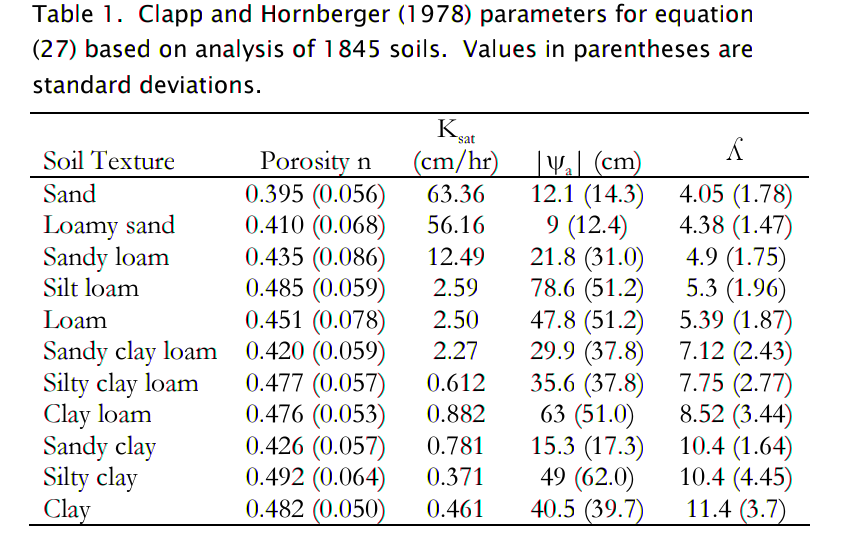
\includegraphics[width=1\textwidth]{./figures/BCParameters.png} 
\caption{Brooke and Corey soil parameters for different texstures. From Dingman, L(2002). Physical Hydrology, 2nd Ed.Prentice Hall, 646p .}\label{fig:BCValues}
\end{figure}
\end{center}


\section{Climate files}

\echo organizes the climate data in a set of binary files containing the necessary information to construct the time dependent spatial fields of atmospheric inputs. All maps related to climate must be placed in the folder identified in the \emph{Clim\_Maps\_Folder} key of the configuration file.

The spatial distribution of climate data is done according to discrete climate zones with unique identifiers that define areas of the domain with constant values for a given climate input. These climate zones can be constructed using Voronoi polygons, using irregular regions following elevation and aspect bands, or simply using a regular orthogonal spatial grid. This information on the climate zones is provided as a CSF PcRaster map. Figure \ref{fig:ClimZone} is an example of a climate zone map using an orthogonal grid.

\begin{center}
\begin{figure}
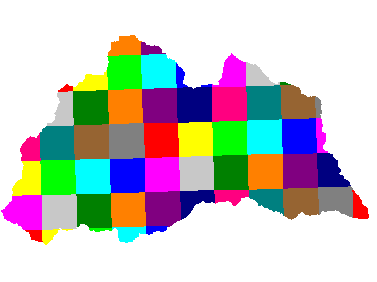
\includegraphics[scale=1]{./figures/ClimateZones.png} 
\caption{Example of a climate zone map using a regular grid to accommodate input form a regional climate model}\label{fig:ClimZone}
\end{figure}
\end{center}


A time series of climate information for each specific climate zone is associated with each of these zones through a unique identifier that links the climate zone and a specific column of the binary climate file.     

\echo reads climate files in a specific binary format that can be constructed from a text file using the \textsf{asc2c} utility provided with \echo. The format of the text file needed to run \textsf{asc2c} is explained below and summarized in box \ref{box:climformat}. Data must be space or tab separated except the first line that must end with a carriage return.  

\begin{center}
\begin{Frame}
\label{box:climformat}
\begin{verbatim}

Comment [up to 256] (character)
NumTimeSteps [1] (integer number)
TimeSteps [NumTimeSteps] (real number)
NumZones [1] (integer number)
ZoneId [NumZones] (integer number)
Data [NumTimeSteps x NumZones] (real number)

\end{verbatim}
\end{Frame}
Box \ref{box:climformat}: ASCII climate file format. The number in square brackets is the number items allowed of the type indicated in parentheses
\end{center}


The first line of the file is a user's comment that typically includes a desciption of the contents of the file such as the what variable is represented in the file (precipitation, air temperature, etc), its source, units, etc. The size of the comment cannot exceed 256 characters including white spaces. The line may be left blank but the line must still exist (i.e. even if there is no information there must be a blank line).
 
The second line is the number of time steps included in the database. It must be a single integer.

The next line identifies the time steps in arbitrary units (e.g. 0.5 1 1.5... hours or 1 2 3 4... days). it is a space- or tab-separated list of real numbers containing exactly \texttt{NumTimeSteps} elements. The elements in this list are read with single precision (32 bits).
 
The next line is the number of spatial climate zones for which a time series is provided in the file. It must be a single integer.
 
The next line lists the climate zone identifiers as per the climate zone map that will be used during the simulations. This list is space- or tab-separated containing exactly \texttt{NumZones} integer numbers.

The final group of numbers contains the actual climate data. It is a matrix of real numbers with \texttt{NumTimeSteps} rows (a row per time step) and \texttt{NumZones} columns (one column per time zone listed in the header). Each column representing data for a zone must be ordered according to the order the zones were listed in the header. Elements in this matrix are read with single precision (32 bits).     

Box \ref{box:climfileex} gives An example of a climate file correctly formatted is 
\mbox


\begin{center}
\begin{Frame}
\label{box:climfileex}
\begin{verbatim}

Windspeed in m/s. Station 1b2. J Doe
4
0.5 1 1.5 2
2 
1 2
2.4 2.1
2.0 2.8
1.9 2.0
0.5 1.2

\end{verbatim}
\end{Frame}
Box \ref{box:climfileex}: Example of ascii climate file with 4 time steps (0.5, 1, 1.5, and 2) and 2 climate zones (1 and 2)
\end{center}

\begin{center}
Table \ref{tab:climvars} File format of vegetation parameters needed to run the vegetation component of \echo
\label{tab:climvars}
\begin{longtable}{|l|l|}
\hline 
\textbf{Variable} & \textbf{Units} \\ 
\hline 
Precipitation & $ms^{1}$ \\ 
\hline 
Average air temperature & $centigrades$ \\ 
\hline 
Maximum air temperature & $centigrades$ \\ 
\hline 
Minimum air temperature & $centigrades$ \\ 
\hline 
Relative Humidity & fraction of saturation \\ 
\hline 
Wind speed & $ms^{1}$ \\ 
\hline 
Incoming long wave radiation & $Wm^{-2}$ \\ 
\hline 
Incoming solar radiation & $Wm^{-2}$ \\ 
\hline 
\end{longtable}
\end{center} 
 
Text files with this format need to be converted into the appropriate binary climate format used by \echo using the provided \textsf{asc2c} utility

\begin{verbatim}
asc2c input_text_file.asc output.bin
\end{verbatim}
 
Where \textsf{input\_text\_file.asc} represents the name of the appropriately formatted text file containing the climate data and \textsf{output.bin} represents the name that \textsf{asc2c} will use to write the resulting binary file. The format of the binary file follows the same structure of the ascii file using 8 bit characters, 32 bit signed integers, and 32 bit signed floats.

Eight climate variables are needed to run \echo, each in its own binary file. \echo expects the data in the files to be in some specific units. Table \ref{tab:climvars} lists the eight needed climate variables and the corresponding units in which the data must be provided.   

Two additional files in CSF PcRaster map format are necessary in \emph{Clim\_Maps\_Folder}, one is a map with the temperature threshold (in $^\circ C$) for rain to snow transition. This map can be constant or the threshold can change in space. The second file is a convenience map of precipitation multiplication factors that permits to manipulate and improve the spatial distribution of precipitation even when using coarse climate zones. The precipitation assigned to a pixel in the climate zone from the corresponding \textit{.bin} file will be multiplied by the factor specified in the same pixel of this map before being used in \echo. 

\section{Forest and species data} 

In this version \echo is designed to simulate evergreen vegetation and a herbaceous understory. It is also designed to broad types of vegetation (e.g.  firs, pines) with a general functional behavior instead of simulating specific species. Multiple vegetation types can be simulated, the number of them is supplied in the \emph{Number\_of\_Species} keyword of the configuration file.

\echo needs two type of information to set up the ecological module: 1) vegetation parameters, and 2)initial condition of the state variables tracked. 

\subsection{Vegetation Parameters file}
The vegetation parameters file must be located in the \emph{Maps\_Folder} folder indicated in the configuration file. The name of the file must be indicated in the \emph{Species\_Parameters} keyword. 

The contents of the file is ascii text that describes the functional characteristics of the different vegetation types that will be included in the simulation. It contains the time-invariant parameters that define the behavior of plants.

The first line of the file contains two tab- or space-separated integers. The first integer indicates the number of vegetation types included in the file. The second integer must be the number 43, which is the number of information items that needs to be supplied for each vegetation type. 

Below the first line there will be a line per vegetation type containing 43 items of information. The format and items of information are listed in Table \ref{tab:vegparams}.

\begin{center}
Table \ref{tab:vegparams}: Format of the vegetation parameters file
\begin{Frame}\label{tab:vegparams}
\begin{verbatim}
line 1: numSpecs	NumParams												
In each line from line 1 to line numSpecs+1: 43 Comma or
tab separated numbers with the following elements:

SpeciesID NPP/GPPRatio	gsmax	CanopyQuantumEffic
MaxForestAge OptimalTemp MaxTemp MinTemp 
FoliageAllocCoef_a	FoliageAllocCoef_b 
StemAllocCoef_a	StemAllocCoef_b	gs_light_coeff	gs_vpd_coeff
lwp_low lwp_high WiltingPnt	SpecificLeafArea
 SpecificRootArea Crown2StemDRat 
TreeShapeParam	WoodDens Fhdmax	Fhdmin LeafTurnoverRate
MaxLeafTurnoverWaterStress LeafTurnoverWaterStressParam
MaxLeafTurnoverTempStress LeafTurnoverTempStressParam
ColdStressParam	RootTurnoverRate MaxCanStorageParam albedo
emissivity	KBeers	CanopyWatEffic sperry_d_par sperry_c_par 
sperry_K_param gsr_param_a vegtype 
DeadGrassLeafTurnoverRate DeadGrassLeafTurnoverTempAdjustment 

\end{verbatim}
\end{Frame}
\end{center} 

\hangindent=0.7cm
\paragraph{SpeciesID}: A unique vegetation identifier (integer).

\hangindent=0.7cm
\paragraph{NPP/GPPRatio}: A NPP to GPP ratio representing a constant respiration loss. Positive real smaller than 1. Typical value around 0.47

\hangindent=0.7cm
\paragraph{gsmax}: Maximum stomatal conductance in $ms^{-1}$. Typical value around 0.006

\hangindent=0.7cm
\paragraph{CanopyQuantumEffic}: Canopy quantum efficiency representing the light use efficiency, in $gCJ^{-1}$ (grams of carbon per absorbed joule of photosynthetically active radiation. Typical value around 0.0000018

\hangindent=0.7cm
\paragraph{MaxForestAge}:  Typical maximum age for the vegetation, in years

\hangindent=0.7cm
\paragraph{OptimalTemp}: Optimal growth temperature for the vegetation type, in degrees C

\hangindent=0.7cm
\paragraph{MaxTemp}: Maximum temperature of comfort for the species, in degrees C

\hangindent=0.7cm
\paragraph{MinTemp}: Minimum temperature of comfort for the species, in degrees C

\hangindent=0.7cm
\paragraph{FoliageAllocCoef\_a}: Foliage allocation coefficient as per 3PG model. Typical value around 2.235 	

\hangindent=0.7cm
\paragraph{FoliageAllocCoef\_b}: Foliage allocation coefficient as per 3PG model. Typical value around 0.006 	

\hangindent=0.7cm
\paragraph{StemAllocCoef\_a}: Stem allocation coefficient as per 3PG model. Typical value around 3.3 	

\hangindent=0.7cm
\paragraph{StemAllocCoef\_b}: Stem allocation coefficient as per 3PG model. Typical value around 0.0000006 	

\hangindent=0.7cm
\paragraph{gs\_light\_coeff}: Parameter controlling stomatal sensitivity to light. Typical value around 300

\hangindent=0.7cm
\paragraph{gs\_vpd\_coeff}: Parameter controlling stomatal sensitivity to vapor pressure deficit. Typical value around 0.002

\hangindent=0.7cm
\paragraph{lwp\_low}: Lowest leaf water potential before stomatal function shuts down. Typical value around -400 m of head

\hangindent=0.7cm
\paragraph{lwp\_high}: Leaf water potential threshold beyond which stomatal efficiency is maximal. Typical value around -7 m of head

\hangindent=0.7cm
\paragraph{WiltingPnt}: Volumetric soil water content at wilting point, dependent on plant and soil characteristics. 

\hangindent=0.7cm
\paragraph{SpecificLeafArea}: Specific leaf area, in $m^2KgC^{-1}$

\hangindent=0.7cm
\paragraph{SpecificRootArea}: Specific root area, in $m^2KgC^{-1}$

\hangindent=0.7cm
\paragraph{Crown2StemDRat}: Allometric parameter controlling the crown to stem diameter ratio as per TreeDyn. 

\hangindent=0.7cm
\paragraph{TreeShapeParam}: Tree shape parameter as per TreeDyn. An often appropriate value is 0.4

\hangindent=0.7cm
\paragraph{WoodDens}: Wood density, in $gCm^{-2}$

\hangindent=0.7cm
\paragraph{Fhdmax}: Maximum allowed ratio of tree height to stem diameter 

\hangindent=0.7cm
\paragraph{Fhdmin}: Minimum allowed ratio of tree height to stem diameter 

\hangindent=0.7cm
\paragraph{LeafTurnoverRate}: Base leaf turnover rate, in $s^{-1}$ 

\hangindent=0.7cm
\paragraph{MaxLeafTurnoverWaterStress}: Maximum leaf turnover rate due to water stress, in $s^{-1}$  

\hangindent=0.7cm
\paragraph{LeafTurnoverWaterStressParam}: Parameter controlling increased leaf turnover due to water stress 

\hangindent=0.7cm
\paragraph{MaxLeafTurnoverTempStress}: Maximum leaf turnover rate due to temperature stress, in $s^{-1}$   

\hangindent=0.7cm
\paragraph{LeafTurnoverTempStressParam}: Parameter controlling increased leaf turnover due to temperature stress 

\hangindent=0.7cm
\paragraph{ColdStressParam}   (degC)

\hangindent=0.7cm
\paragraph{RootTurnoverRate}: Base root turnover rate, in $s^{-1}$

\hangindent=0.7cm
\paragraph{MaxCanStorageParam}: Maximum water storage capacity of the canopy, in $m$

\hangindent=0.7cm
\paragraph{albedo}: Albedo of vegetation

\hangindent=0.7cm
\paragraph{emissivity}: Emissivity of vegetation

\hangindent=0.7cm
\paragraph{KBeers}: Light extinction coefficient for the canopy as per Beer's law

\hangindent=0.7cm
\paragraph{CanopyWatEffic}: Water use efficiency of the canopy, in terms of grams of carbon assimilated per meter of transpired water, $gCm^{-1}$

\hangindent=0.7cm
\paragraph{sperry\_d\_param}: Normalization denominator factor in Sperry's model of plant hydraulic conductance, in $m$. Typical value 204 m

\paragraph{sperry\_c\_param}: Exponent parameter c in Sperry's model of plant hydraulic conductance. Typical value 2 m

\paragraph{sperry\_K\_param}: Hydraulic conductivity of plant tissue, in $ms^{-1}$. Typical value 1.15-e6 $ms^{-1}$

\paragraph{gsr\_param\_a}: Parameter that controls the loss of conductance in the rhizosphere as soil dries. Typical value 8

\hangindent=0.7cm
\paragraph{is\_grass}: Switch that indicates if the vegetation type is herbaceous (1) or not (0)

\hangindent=0.7cm
\paragraph{DeadGrassLeafTurnoverRate}: Base Rate of decomposition of dry grass leaves,  $s^{-1}$. The value is used only if \emph{is\_grass}=1 although a value needs to be supplied in all cases 

\hangindent=0.7cm
\paragraph{DeadGrassLeafTurnoverTempAdjustment}: Temperature threshold that triggers the decomposition of dry grass leaves,  $\deg C$. The value is used only if \emph{is\_grass}=1 although a value needs to be supplied in all cases    
 

\subsection{Initial conditions for vegetation state variables}

Information on the density of trees, relative canopy cover, root density, leaf area index, vegetation age, vegetation effective height, and tree basal area is necessary to initialize the status of vegetation. There is two ways to provide this information: using tables and using maps. 

\subsection{Initialization using tables}
Initialization of the state variables for vegetation using tables is often easier during the first model run. \echo can be initialized with tables by setting \emph{Species\_State\_Variable\_Input\_Method} = tables in the configuration file. 

This type of initialization relies on the concept of \textit{'vegetation patches'}, which are discrete, arbitrarily-shaped regions in the study area where vegetation is initialized with constant values. A patch can have multiple vegetation types, each identified with the \emph{SpeciesID} listed in the vegetation parameter file.

Patches are given to \echo as a map in the \emph{'ForestPatches'} keyword of the configuration file. This map must be included in the \emph{Maps\_Folder} folder indicated in the configuration file. The map contains at least one discrete region (patch) identified with an integer. Please note that patches need not be continuous. A patch can be composed of different disconnected small regions scattered through the domain with the same integer identifier. 

The initialization of vegetation types in each path is done through a number of ascii tables with a format described below. The tables must be placed in the \emph{Maps\_Folder} folder indicated in the configuration file and the names for each variable paired with the appropriate key in the configuration file. A description of the tables is given below

\paragraph{Species\_Proportion\_Table}: Table containing the proportion of each patch that is occupied by each vegetation type. In the current version of the model this is a time-invariant variable since there is no vegetation dispersal and encroachment module. If a vegetation type does not exist for a patch, indicate a zero in the column for that species in a patch.

\paragraph{Species\_StemDensity\_Table }: Table containing the tree density of each vegetation type in their share of patch, in trees per sq. meter. In the current version of the model this is a time-invariant variable since there is no vegetation dispersal and encroachment module.

\paragraph{Species\_LAI\_Table  }: Table containing the initial LAI of each vegetation type. note that LAI is defined as the area of leaves over the projected canopy area and not area of leaves over patch or pixel area. 

\paragraph{Species\_AGE\_Table  }: Table containing the average age of trees of each vegetation type in each patch. In years. 

\paragraph{Species\_BasalArea\_Table  }: Table containing the total basal area of each type of vegetation in each patch, in square meters.

\paragraph{Species\_Height\_table  }: Table containing the effective height of each type of vegetation in each patch, in meters.

\paragraph{Species\_RootMass\_table  }: Table containing the average root mass of each type of vegetation in each patch, in grams per square meters.

All tables have identical format as described in Table \ref{tab:vegvars}.

\begin{center}
Table \ref{tab:vegvars}: Format of the vegetation variables file
\begin{Frame}
\label{tab:vegvars}
\begin{verbatim}
line 1: numPatches	NumSpecies+1
In each line from line 1 to line numPatches+1: PatchID
followed by NumSpecies comma or tab separated
numbers with initial information on vegetation variables.
The information for each vegetation type is listed in 
the same order they appear in the vegetation parameter
file.
\end{verbatim}
\end{Frame}
\end{center} 

\paragraph{numPatches}: Number of patches with unique identifiers in file associated to \emph{ForestPatches}. 

\paragraph{NumSpecies}: Is the number o simulated vegetation types.

\paragraph{PatchID}: The unique integer identifier for the vegetation patch as identified in the patch map. \\

\textbf{Important:} The information for the vegetation type is introduced in the order in which the vegetation types are listed in the vegetation parameterfile (i.e. first number after the \emph{PatchID} item corresponds to the topmost vegetation type listed in the vegetation parameter file, and so on. 


\subsection{Initialization using maps}

If distributed information is available to initialize the vegetation variables or if a complete run has already been performed it is possible to initialize the variables using maps instead of tables and provide variability within each patch.

To initialize the vegetation variables this way set \emph{Species\_State\_Variable\_Input\_Method} = maps in the configuration file. With the configuration, \echo will look for the following maps in the folder specified in  \emph{Maps\_Folder}:

The species are identifying by an index within square brackets in the file name. The index starts at 0, which identifying the topmost vegetation type identifyed in the vegetation parameter file (e.g. for a run with two vegetation types the leaf area index is initialized with two maps, emp{lai[0].map} and \emph{lai[1].map},  corresponding to the first and second vegetation types listed in the vegetation parameter file).  

\paragraph{p[0,...,NumSpecies-1].map}: One map per vegetation type included in the simulation. The map contains the proportion of each pixel occupied by the vegetation type identifying by the index in the file name.

\paragraph{root[0].map}: One map per vegetation type included in the simulation. The map contains the root mass of the vegetation type identifying by the index in the file name, in $gm{-2}$
 
\paragraph{ntr[0,...,NumSpecies-1].map}: One map per vegetation type included in the simulation. The map contains density of trees in the area of each pixel ocuppied by the vegetation type identified by the index in the file name. Trees per sq. meter.

\paragraph{lai[0,...,NumSpecies-1].map}: One map per vegetation type included in the simulation. The map contains the initial leaf area index in each pixel of the vegetation type identified by the index in the file name.

\paragraph{hgt[0,...,NumSpecies-1].map}: One map per vegetation type included in the simulation. The map contains the effective height in each pixel of the vegetation type identified by the index in the file name. In meters. 

\paragraph{bas[0,...,NumSpecies-1].map}: One map per vegetation type included in the simulation. The map contains the total basal area in each pixel of the vegetation type identified by the index in the file name. In sq. meters.

\paragraph{age[0,...,NumSpecies-1].map}: One map per vegetation type included in the simulation. The map contains the age in each pixel of the vegetation type identified by the index in the file name. In years.\\

A way to produce these maps is to turn on the reporting flag for these maps during an initial run of \echo using tables. Then rename the last time step of the corresponding files in the results folder with the appropriate names and copy these files to the maps folder. The case study included in this manual explains how initialize the model using this technique. 
